%%%%%%%%%%%%%%%%%%%%%%%%%%%%%%%%%%%%%%%%%%%%%%%%%%%%%%%%%%%%%%%%%%%%%%%%
%%% documentclass and packages
%%%%%%%%%%%%%%%%%%%%%%%%%%%%%%%%%%%%%%%%%%%%%%%%%%%%%%%%%%%%%%%%%%%%%%%%
\RequirePackage{atbegshi}           % workaround for newer PGF versions
%\documentclass[hyperref={pdfpagelabels=false}]{beamer}
%\documentclass[aspectratio=1610,t]{beamer}
\documentclass[t]{beamer}
% https://sourceforge.net/tracker/index.php?func=detail&aid=1848912&group_id=92412&atid=600660
\usepackage{lmodern}
\usepackage[T1]{fontenc}
\usepackage[utf8]{inputenc}
\usepackage{textcomp}

\usepackage[english]{babel}
\usepackage[babel,english=american,german=guillemets]{csquotes}	% french
\usepackage{microtype}
\usepackage{tikz}
\usetikzlibrary{graphs}
\usetikzlibrary{quotes}
\usetikzlibrary{shapes.geometric}
\usetikzlibrary{shapes.misc}

% colors for listings
\definecolor{lightergray}{gray}{.95}
\definecolor{darkblue}{rgb}{0,0,0.5}
\definecolor{darkgreen}{rgb}{0,0.5,0}
\definecolor{darkred}{rgb}{0.5,0,0}
\definecolor{darkerblue}{rgb}{0,0,0.4}
\definecolor{darkergreen}{rgb}{0,0.4,0}
\definecolor{darkerred}{rgb}{0.4,0,0}

\usepackage{listings}
% \lstloadlanguages{HTML,XML}
\lstset{%
    basicstyle=\ttfamily\small\mdseries,
    keywordstyle=\bfseries\color{darkblue},
    identifierstyle=,
    commentstyle=\color{darkgray},
    stringstyle=\itshape\color{darkred},
    frame=none,
    showstringspaces=false,
    tabsize=4,
    backgroundcolor=\color{lightergray},
}

%%%%%%%%%%%%%%%%%%%%%%%%%%%%%%%%%%%%%%%%%%%%%%%%%%%%%%%%%%%%%%%%%%%%%%%%
%%% macros
%%%%%%%%%%%%%%%%%%%%%%%%%%%%%%%%%%%%%%%%%%%%%%%%%%%%%%%%%%%%%%%%%%%%%%%%

% strong emphasis (like in HTML)
\makeatletter
\newcommand{\strong}[1]{\@strong{#1}}
\newcommand{\@@strong}[1]{\textbf{\let\@strong\@@@strong#1}}
\newcommand{\@@@strong}[1]{\textnormal{\let\@strong\@@strong#1}}
\let\@strong\@@strong
\makeatother

\newcommand*{\greenemph}[1]{%
    \tikz[baseline]
        \node[%
            rectangle,
            fill=green!80,
            rounded corners=0.8mm,
            inner sep=0.8mm,
            anchor=base
        ]{#1};%
}

%%%%%%%%%%%%%%%%%%%%%%%%%%%%%%%%%%%%%%%%%%%%%%%%%%%%%%%%%%%%%%%%%%%%%%%%
%%% preparations for beamer
%%%%%%%%%%%%%%%%%%%%%%%%%%%%%%%%%%%%%%%%%%%%%%%%%%%%%%%%%%%%%%%%%%%%%%%%
\useinnertheme{default}
\useoutertheme{infolines}
%\usecolortheme[rgb={0.28,0.37,0.52}]{structure}
\usecolortheme[rgb={0.18,0.23,0.33}]{structure}
%\usecolortheme{beaver}
\usefonttheme{structurebold}

%%% Ränder vergrößern für's Café Central
%\setbeamersize{text margin left=1.2cm}
%\setbeamersize{text margin right=1.2cm}

%%% let hyperlinks look like hyperlinks
\hypersetup{%
    colorlinks=true,
    linkcolor=black,
    urlcolor=darkblue
}

%%%%%%%%%%%%%%%%%%%%%%%%%%%%%%%%%%%%%%%%%%%%%%%%%%%%%%%%%%%%%%%%%%%%%%%%
%%% images
%%%%%%%%%%%%%%%%%%%%%%%%%%%%%%%%%%%%%%%%%%%%%%%%%%%%%%%%%%%%%%%%%%%%%%%%

%%%%%%%%%%%%%%%%%%%%%%%%%%%%%%%%%%%%%%%%%%%%%%%%%%%%%%%%%%%%%%%%%%%%%%%%
%%% title, author, date
%%%%%%%%%%%%%%%%%%%%%%%%%%%%%%%%%%%%%%%%%%%%%%%%%%%%%%%%%%%%%%%%%%%%%%%%
\title[netfilter]{Linux Netfilter}
%\subtitle{Eine nachhaltigere und umweltfreundlichere Informationstechnologie ist möglich …}
\author{Alexander Dahl}
\institute[blog.antiblau.de]{\url{http://blog.antiblau.de/}}
\date{2019-08-21}
%\subject{subj}
%\keywords{FLOSS}

%%%%%%%%%%%%%%%%%%%%%%%%%%%%%%%%%%%%%%%%%%%%%%%%%%%%%%%%%%%%%%%%%%%%%%%%
%%% document
%%%%%%%%%%%%%%%%%%%%%%%%%%%%%%%%%%%%%%%%%%%%%%%%%%%%%%%%%%%%%%%%%%%%%%%%
\begin{document}

\begin{frame}
    \titlepage
\end{frame}

%\begin{frame}
%    \tableofcontents
%\end{frame}

\section{Was?}

\begin{frame}{Linux Netfilter Packet Flow}
    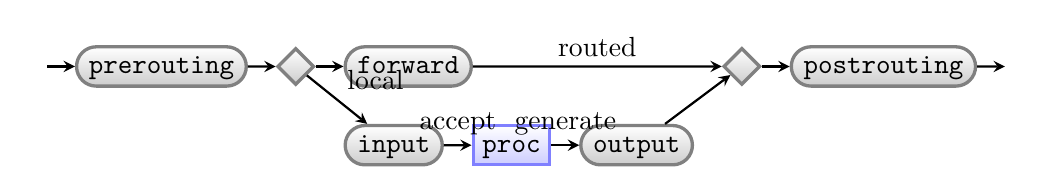
\begin{tikzpicture}[%
        %node distance=15mm,
        chain/.style={
            % the shape:
            rounded rectangle,
            % the rest:
            very thick,
            draw=black!50,
            top color=white,
            bottom color=black!20,
            font=\ttfamily,
            text height=1.5ex,
            text depth=.25ex,
        },
        decision/.style={
            diamond,
            very thick,
            draw=black!50,
            top color=white,
            bottom color=black!20,
            font=\ttfamily
        },
        proc/.style={
            very thick,
            draw=blue!50,
            top color=white,
            bottom color=blue!20,
            font=\ttfamily,
            text height=1.5ex,
            text depth=.25ex,
        },
        >=stealth, thick
    ]

    \graph [grow right sep, simple] {
        / -> prerouting[chain] -> eins/""[decision] -> { 
            forward[<"routed",chain],
            input[>"local",chain] -> ["accept"] proc[proc] -> ["generate"] output[chain]
        } -> zwei/""[decision] -> postrouting[chain] -> /;
    };

\end{tikzpicture}

% vim: ft=tex

\end{frame}

\section{Wie?}

\begin{frame}{Userspace Utilities}
    \begin{itemize}
        \item iptables
        \item nftables
    \end{itemize}
\end{frame}

\section*{Was noch?}

\begin{frame}{Die vorletzte Folie}
    \begin{block}{Kontakt}
        \begin{description}[Twitter]
            \item [E-Mail] \href{mailto:post@lespocky.de}{post@lespocky.de}
            \item [WWW] \href{http://www.lespocky.de/}{lespocky.de} or
                    \href{http://blog.antiblau.de/}{blog.antiblau.de}
            \item [Twitter] \href{https://twitter.com/LeSpocky}{@LeSpocky}
        \end{description}
    \end{block}
    \begin{block}{Folien}
        \begin{itemize}
            \item \texttt{hg clone https://bitbucket.org/lespocky/talks}
        \end{itemize}
    \end{block}
    \begin{block}{Lizenz}
        Dieses Werk ist lizenziert unter einer
        \href{http://creativecommons.org/licenses/by-sa/4.0/}{Creative Commons
        Namensnennung - Weitergabe unter gleichen Bedingungen 4.0 International
        Lizenz}.
    \end{block}
\end{frame}

%\appendix

\begin{frame}{Lizenzen}
    \begin{block}{The Linux Mascot}
        Penguin Tux by \href{mailto:lewing@isc.tamu.edu}{Larry Ewing}
        and \href{http://isc.tamu.edu/~lewing/linux/}{The GIMP},
        vectorized by \href{http://www.home.unix-ag.org/simon/}{Simon Budig},
        converted to TikZ by
        \href{http://www.texample.net/weblog/2012/apr/28/tux-tex-tikz/}{Stefan Kottwitz}.
    \end{block}
\end{frame}

\end{document}
